
\section{\SCONE Architecture}
\label{sec:method}

We propose to augment a standard transformer model with an additional f-gram embedding layer. \Cref{fig:method_overview} provides a high-level overview of the approach. We first construct a set $\Vfgram \subseteq \Vtoken^{[2, K]} := \bigcup_{n=2}^K \Vtoken^{n}$ consisting of frequently occurring \ngram{n}s of length up to $K$, which we refer to as \emph{f-grams}. Throughout this paper, $K$ denotes the maximum length of f-grams considered. 
To construct $\Vfgram$, we use an efficient implementation that requires only $K-1$ linear scans over the training corpus, as detailed in \Cref{subsec:key_discovery}; the formal construction is described in \Cref{alg:n-gram-vocab} (\Cref{sec:add_algorithms}).

{\renewcommand{\baselinestretch}{1.22}\selectfont
\begin{algorithm}[t]
\small
\caption{\SCONE method $F_{\cT, \Vfgram, \train{\Afgram} | \infer{\cF}}$.}
\label{alg:scone-first-stage}
\begin{algorithmic}
\STATE \begin{itemize}[itemsep=-2pt]
    \item $\cT : \Vtoken \to \R^d$: token embedding layer.
    \item $\Vfgram \subseteq \Vtoken^{\le K}$: set of f-grams.
    \item \textbf{\textsc{Training}}: f-gram transformer model
    \begin{itemize}[leftmargin=8mm,label=$\triangleright$,itemsep=-3pt,topsep=-4pt]
        \item \train{$\Afgram : (\R^d)^{\le K} \to \R^d$}.
    \end{itemize}
    \item \textbf{\textsc{Inference}}: f-gram embedding layer
    \begin{itemize}[leftmargin=8mm,label=$\triangleright$,itemsep=-3pt,topsep=-4pt]
        \item \infer{$\cF : \Vfgram \to \R^d$}.
    \end{itemize}
\end{itemize}
\STATE {\bf Input:} A sequence $(\sigma_1, \ldots, \sigma_m) \in \Vtoken^m$ of tokens.
\STATE {\bf Output:} Embeddings $(\be_1, \ldots, \be_m) \in (\mathbb{R}^d)^m$.
\FOR{$i = 1, \ldots, m$}
    \STATE $j \gets$ smallest $j' < i$ such that $(\sigma_{j'}, \ldots, \sigma_i) \in \Vfgram$ if such a $j'$ exists, otherwise $i$.
    \IF{$j = i$}
        \STATE $\be_i \gets \cT(\sigma_i)$
    \ELSE
        \STATE $\be_i \gets \begin{cases}
            \Afgram(\cT(\sigma_{j}), \ldots, \cT(\sigma_i)) & \text{at training,}\\
            \cF(\sigma_{j}, \ldots, \sigma_i) & \text{at inference.}
        \end{cases}$
    \ENDIF
\ENDFOR
\RETURN $(\be_1, \ldots, \be_m)$
\end{algorithmic}
\end{algorithm}
}

Next, we define the \SCONE method, which maps a given sequence of tokens to a sequence of embeddings. \SCONE behaves differently during training and inference, as described in \Cref{alg:scone-first-stage}. During training, it is parameterized by an f-gram transformer model $\Afgram : (\R^d)^{\le K} \to \R^d$, which takes an f-gram as  input and uses the output embedding of the final token as the embedding for that f-gram. During inference, in contrast, it is parameterized by an f-gram embedding layer $\cF : \Vfgram \to \R^d$, a key--value store that directly maps each f-gram to its precomputed embedding. This embedding layer is implemented by caching the outputs of $\Afgram$ for all f-grams in $\Vfgram$ and storing them in off-accelerator memory.

The embeddings produced by \SCONE are passed to a standard transformer model $\Amain$, referred to as the \emph{main model}. This is followed by a prediction head $\cD : \R^d \to \Delta_{\Vtoken}$. Together, these components form the end-to-end process for next-word prediction with \SCONE. We present the full description in \Cref{alg:scone-model} (\Cref{sec:add_algorithms}).



In the rest of this section, we will discuss the motivation behind the design chocies of \SCONE and provide further implementation details.


\subsection{\boldmath BPE-Style Discovery of f-grams}
\label{subsec:key_discovery}


\begin{wrapfigure}{r}{0.5\textwidth}
  \centering
  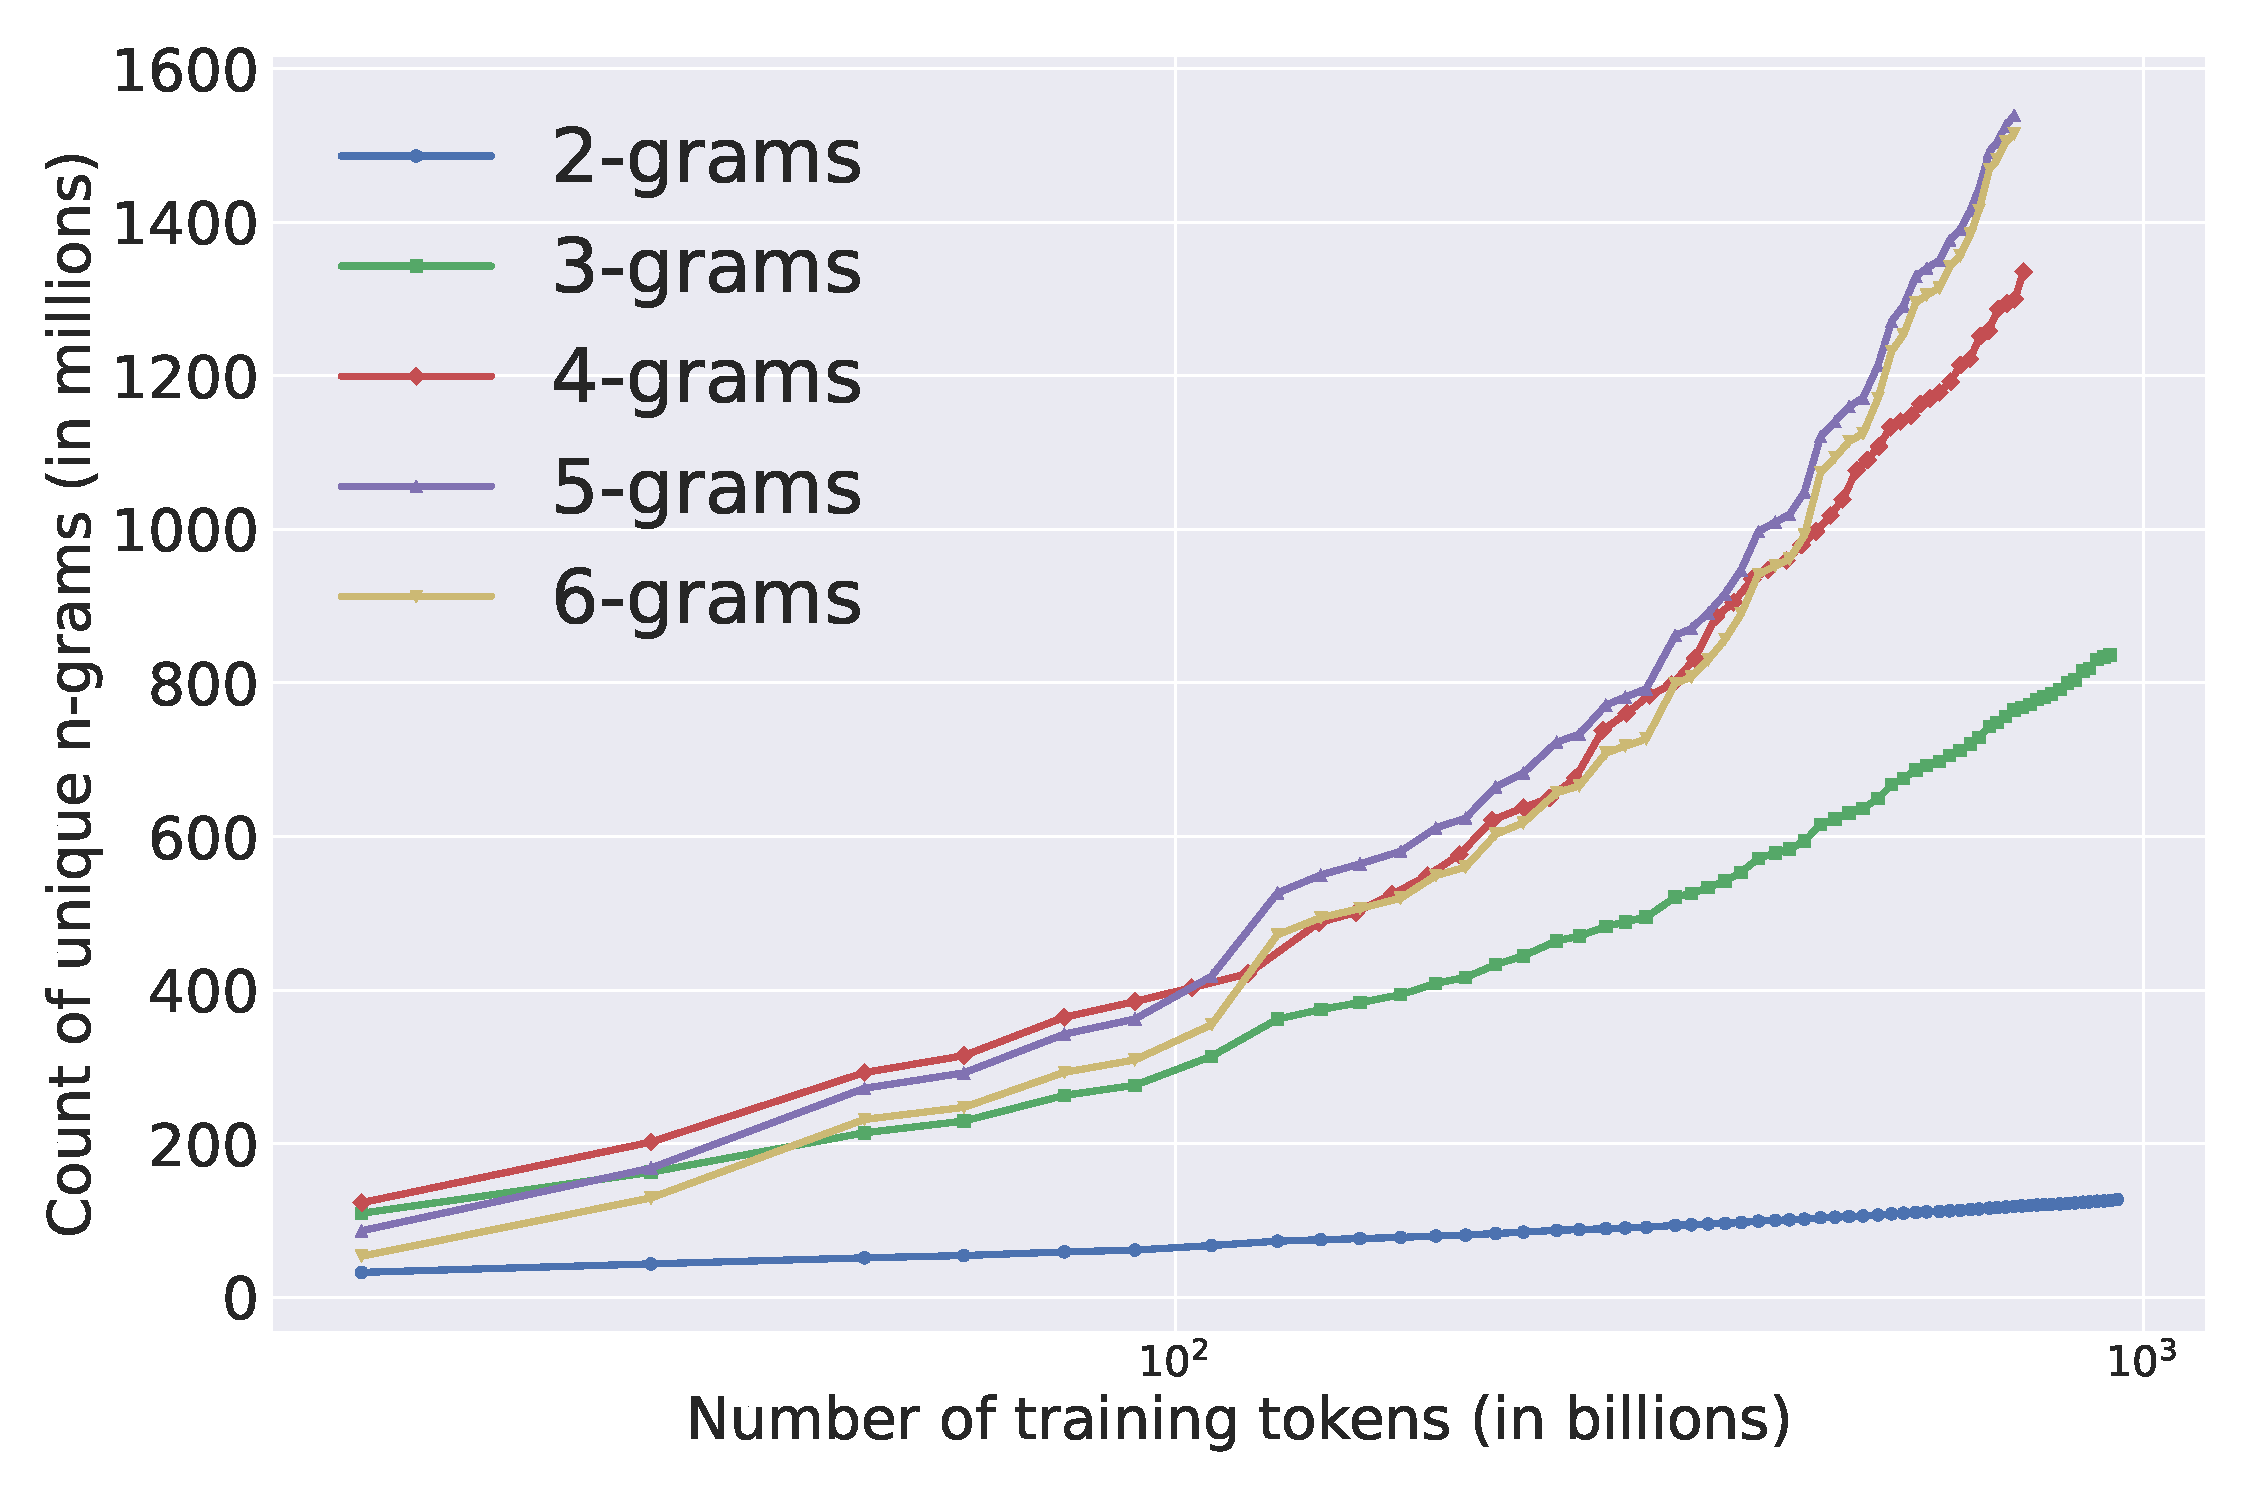
\includegraphics[width=0.48\textwidth]{figs/olmo_num_ngrams.pdf}
  \caption{Number of unique $2$- to $6$-grams appearing at least five times. We uniformly sample tokenized sequences from Dolma \citep{soldaini2024dolma} to vary the corpus size.}
  \label{fig:num_ngrams}
\end{wrapfigure}


The construction of $\Vfgram$, outlined in \Cref{alg:n-gram-vocab} (\Cref{sec:add_algorithms}), can be implemented efficiently with $K-1$ linear scans over the training corpus. 
We perform one scan for each $n \in [2, K]$, starting with \ngram{2}s.
In subsequent scans, we impose a minimum frequency threshold of 5 to reduce memory usage. At the $(n+1)${th} scan, the set of \ngram{n}s from the previous scan allows us to skip any \ngram{(n+1)} candidates that cannot meet the minimum threshold. Specifically, if an \ngram{(n+1)} surpasses the threshold, its $n$-suffix or prefix must appear at least as many times. \Cref{fig:num_ngrams} shows how the number of unique \ngram{n}s (up to \ngram{6}s) grows as the training corpus scales from a few billion to one trillion tokens. Finally, all found \ngram{n}s (for $n \in [2, K]$) are ranked by frequency, and the top ones are selected to comprise $\Vfgram$.

Our procedure for counting and ranking \ngram{n}s is analogous to continuing the training of a BPE tokenizer on an existing vocabulary. In each BPE iteration \citep{gage1994new,sennrich2015neural}, the frequencies of all token pairs (\ngram{2}s) are counted, and the most frequent pair is merged to form a new token, expanding the vocabulary by one. However, merging and recounting pairs repeatedly to obtain a large number of f-grams is prohibitively expensive for large training corpora. Instead, we simply collect and sort all \ngram{n}s up to a small constant $K$.

\subsection{\boldmath Learning f-gram Embeddings with $\Afgram$}
\label{subsec:train_embedding}

We motivate the use of $\Afgram$ by contrasting it with the alternative of directly backpropagating gradients to a large embedding table.
The direct approach fails to exploit dependencies between \ngram{n}s, leading to fewer updates per embedding. We observed this by pretraining GPT-2 models with vocabulary sizes ranging from 32K to 2M. As vocabulary size increases, embedding updates become sparser, eventually degrading performance. For example, when training on 100M tokens, 97.6\% of tokens in a 32K vocabulary receive more than 100 updates, compared to only 7.3\% in a 2M vocabulary (\Cref{sec:scale_vocab}).
This sparsity makes it difficult to train a large embedding table through direct gradient updates.
\SCONE addresses this by parameterizing embeddings with an f-gram transformer $\Afgram$, avoiding the sparse update problem. 

Additionally, $\Afgram$ removes the need to instantiate a full embedding table during training, a requirement that would otherwise strain accelerator memory. This is because, unlike inference, where next-word prediction is largely sequential, training parallelizes computation across the sequence dimension, demanding much higher token throughput. Moreover, during training, embeddings must be updated  frequently, whereas inference only requires read access. Together, these factors make it difficult to offload the embedding layer from accelerators during training. As a result, avoiding full-table instantiation is crucial for scaling the embedding layer to extremely large sizes.



\SCONE jointly trains the $\Afgram$ model with the main model $\Amain$ and the token embedding layer $\cT$. This overcomes the sparse updates issue but also introduces additional compute costs. For each $\omega\in\Vfgram$, the computation is the same as that of  processing a short sequence of length $|\omega|$ through a standard transformer. Since $|\omega|$ is a small constant, the primary overhead comes from the feed-forward layer. In our experiments (\Cref{sec:exps_openwebtext}), we account for this overhead in one of two ways: (1) by training baseline models long enough to reach near-convergence at a fixed model size, ensuring that additional training compute would yield minimal gains; or (2) by reducing the number of training tokens for models using \SCONE so that their total training FLOPS match those of the baselines.


During inference, the f-gram embedding layer $\cF$ can be precomputed and stored in a lookup table, offloaded to system main memory or secondary storage while still permitting efficient retrieval. Meanwhile, the token embedding layer $\cT$ remains on the accelerator for decoding. In \Cref{subsec:inference_cost}, we evaluate the  query latency and space usage of the f-gram embedding layer under various configurations.  We show that the latency is not a bottleneck for language model inference and the space costs are low due to the use of relatively inexpensive system memory and solid-state drives.







